
	
	\subsection{Empirical Orthogonal Function Analysis}
	\label{subsec:EOF}
	
Empirical Orthogonal Function (EOF) Analysis is a common and widely used statistical technique in atmospheric science for analysing data in high dimensional phase spaces.
The objective is to structure, to simplify  and especially to find in place of the ordinary original variables $x_i(t)$ a relatively small number of new independent variables $u_i(t)$  , which represent as much of the original data sets information as possible. For this reason, a new set of orthogonal coordinate axes $\bm{e_{i}^u}$ instead of the ordinary and often more intuitive axes $\bm{e_{i}^x}$ has to be found, in which to examine the data \cite{Wilks2006}??. 


Loosely speaking ,the desirable characteristics of the new orthogonal coordinate axis are given in such a way that:
\begin{itemize}
	\item the maximum possible amount of variance or variation within the data set can be explained along the 	axis $\bm{e_{1}^u}$ (with new coordinates $u_1(t)$)
	\item the maximum possible amount of remaining variance of the data set can be explained along the subsequent axis $\bm{e_{2}^u}$  
	\item and so forth for the remaining axis $\bm{e_{i}^u}$,
\end{itemize}
subjected to the condition, that the new variables $u_i(t)$ are uncorrelated with the variables having lower indices.\\
In contrast to other analysing and transformation techniques, such as Fourier Transforms or Taylor expansions, in which fixed sinusoidal or polynomial coordinate systems are used, the coordinate axes for an EOF analysis have to be identified uniquely for each specific data set.


		\subsubsection{Basic principle in two dimensions}
		\label{subsubsec:2d-case}
		
 The general procedure of EOF analysis can be best visualized and illustrated in the two dimensional case. For this reason, we will consider a two dimensional phase space with two variables $x_1$ and $x_2$ measured simultaneously at certain times, which for instance may be associated with two temperature measurements at two different locations. %As mentioned before, the main purpose of EOF analysis is to find a new set of %coordinate axes, which represent a large amount of variance of the data set.
In figure \ref{fig:EOF_2d}, the two variables $x_1$ and $x_2$ reveal a strong positive correlation. Instead of using the original coordinate system $\bm{e_{1}^x}$ and $\bm{e_{2}^x}$, which may be associated with the two variables $x_1$ and $x_2$, this system may be rotated for obtaining a new one with variables $u_1$ and $u_2$ and with new orthogonal coordinate axes $\bm{e_{1}^u}$ and $\bm{e_{2}^u}$. As depicted in figure \ref{fig:EOF_2d} (right), displaying the data set in the new $u$-coordinates shows, that most variance or spread of the data set is represented along the $\bm{e_{1}^u}$ axis. The remaining small amount of variance is explained along the orthogonal axes $\bm{e_{2}^u}$.\\
Thus it is obvious, that the initial 2-dimensional ??structure of the data set, can be reduced to a 1-dimensional perspective by just using the new variable $u_1$ , at the expanse of loosing a certain amount of information about the data set.

\begin{figure}
	\centering
		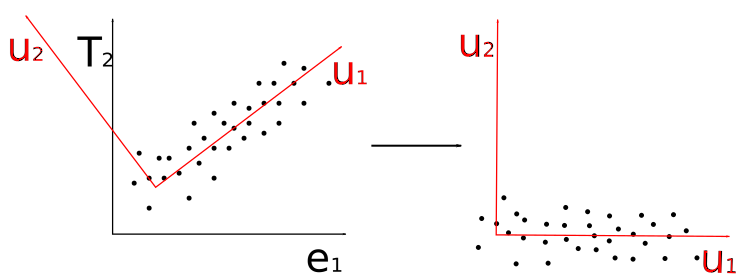
\includegraphics[scale=0.7]{pictures/EOF_2d}
		\caption{Illustration of the basic principle of an EOF analysis: A data set, which is initially represented in an intuitive $x$-coordinate system, may be examined in a new coordinate system with axes $\bm{e_{1}^u}$ and $\bm{e_{2}^u}$ and variables $u_1$ and $u_2$.....  } \label{fig:EOF_2d}
\end{figure}

		\subsubsection{Extension and Generalisation to higher dimensions}
EOF analysis reveals its greatest power, when it comes to analysing  high dimensional data sets, which are rather hard to visualize and structure due to the large number of necessary variables $x_i$.
For this reason, we will extend and generalise the previous considerations to higher N-dimensional phase spaces, which is the general case for a time series of climatic variables $x$ (e.g. sea surface temperature, pressure) defined on $N$ grid points around the globe and measured at $T$ different times $t_k$. (Thus we suppose, that $x$ is given at $N$ grid points at $T$ different time steps.) The climatic variable $x$ at a specific grid point $i=1,...,N$ at time $t_k$ ($k=1,2,...,T)$ is denoted by $x_i(t_k)$.
, which may be summarized at time $t_k$ in  vector notation as

\begin{align*}
	\bm{x(t_k)}=(x_0(t_k),x_1(t_k),...,x_N(t_k)).
\end{align*}
The original and most intuitive basis vectors are thus for instance given by $\bm{e_1^x}=(1,0,0,...,0)$, $\bm{e_2^x}=(0,1,0,...,0)$  with respective coordinates $x_1(t_k)$,$x_2(t_k)$ and so forth.
The objective is to find a new and unique coordinate system, which axes $\bm{e_i^u}$ are linear combinations of the originally defined axis $\bm{e_i^x}$ (i=1,...N) and which have the properties of explaining successively the most variance, as mentioned before in \ref{subsec:EOF}. The corresponding new time dependent variables $u_i(t_k)$ are related to the initial  basis vectors  $\bm{e_i^x}$  by the projection relation 
\begin{align*}\label{eq:projection}
u_i(t_k)=\bm{e_{i}^u} \bm{x}(t_k)= \sum\limits_{j=1}^N e_{ij}^u x_j(t_k). 
\end{align*}

In order to determine such a coordinate system $\bm{e_i^u}$, the covariance matrix $\bm{\underline{S}^x}$ of the $N$-dimensional time series $\bm{x}(t)$ has to be calculated, which components are defined as

\begin{align*}
	S^x_{ij}&=\text{E}[(x_i(t)-\mu_i)(x_j(t)-\mu_j)]\\
		&=\frac{1}{T} \sum\limits_{k=1}^T [(x_i(t_k)-\mu_i)(x_j(t_k)-\mu_j)]
\end{align*}

where $\mu_i$ denotes the time averaged expectation value at grid point $i$, which is given by

\begin{align*}
	\mu_i=\frac{1}{T}\sum\limits_{k=1}^Tx_i(t_k)	
\end{align*}

and the $x$-index signifies that the matrix is given in initial $x$ coordinates.

%The objective is to find a set of more complex basis vectors $e_i^u$ with respective %new coordinates $u_m$, which are related to the original simple basis vectors and %coordinates by the projection relation
%\begin{align*}
%u_m=\sum e_{mk}^u x_k e_{mk}^x 
%\end{align*}

It has been shown, that the desired new coordinate axes $\bm{e_i^u}$ are given by the eigenvectors of the covariance matrix $\bm{\underline{S}^x}$, which explain the highest possible amount of variance successively (cf. \ref{subsec:EOF}).
Since the covariance matrix $S_x$ is symmetric, its eigenvectors and thus the new coordinate axes $\bm{e_i^u}$ are orthogonal as required and its eigenvalues $\lambda_i$ are reel.
Transforming a symmetric matrix into a representation in its Eigenbasis always implies, that the result is a diagonal matrix. For this reason, the covariance matrix $\bm{\underline{S}^u}$ represented in the new coordinate system $\bm{e_i^u}$ (or Eigenbasis) has the shape

\[
\bm{\underline{S}^u}=
  \begin{pmatrix}
    \lambda_1 & 0 & \dots & 0 \\
    0 & \lambda_2 & \dots & 0 \\
    \vdots & \vdots & \ddots & \vdots \\
    0 & 0 & \dots & \lambda_N
  \end{pmatrix}
  .
\]
As the off-diagonal entries are zero, the new variables $u_i$, in which to represent the data and which are obtained according to equation \ref{eq:projection}, are uncorrelated with each other.\\
Furthermore, the respective reel valued eigenvalues $\lambda_i$ characterise the variance along the respective axis. The fraction of explained variance $\sigma_i^2$ along along an axis $\bm{e_{i}^u}$ is proportional to its respective eigenvalue $\lambda_i$ and given by the relation

\begin{align*}
	\sigma_i^2=\frac{\lambda_i}{\sum\limits_{j=1}^N \lambda_j}
\end{align*}


The new variables $u_i(t_k)$ are commonly called \textit{Principal Components} (PC) and the respective coordinate axes $\bm{e_{i}^u}$ are called \textit{Empirical Orthogonal Functions} (EOF).\\
Since vectors of different length, which are aligned into the same direction might act as eigenvectors of the correlation matrix $\bm{\underline{S}^x}$,there exist different scaling conventions for the EOFs and the corresponding PCs. For the following considerations(,) we will define the EOFs in such a way that the respective PC time series has unit variance.

		\subsection{Application to climatic data}
Since EOFs provide the most efficient set of orthogonal functions, in which to represent a given fraction of the variance of meteorological fields with a minimum number of coefficient (PCs), EOF analysis has been extensively used as an aid in climatological investigations and especially to identify the most dominant patterns of variability in the atmosphere \cite{Kidson1975}(Wallace and Gutzler 1981). For this reason, it has been shown that EOF analysis serves as a useful tool for identifying and characterising atmospheric oscillation and teleconnection patterns around the globe in many climatic variables \cite{Rogers1982} \cite{Thompson2000}??. Thus, 
For examining the structure and the temporal evolution of the SAM we use monthly geopotential height fields for specific pressure levels of the ERA-Interim reanalysis set between 20$^\circ$S and 88$^\circ$S and for the period 1979-2016. (As mentioned in ..) The horizontal resolution of the provided data is 1$^\circ$ along each latitudes and 1.77$^\circ$ along each longitude resulting in a phase space with 6300 dimensions. 
Since we are interested in deviation from the mean annual cycle
Due to the fact that grid points are equally spaced on a regular latitude-longitude grid, the number of grid points per unit area increases with higher latitudes(,)
as the meridians converge at the poles. Therefore, high latitude features would be amplified and mid latitude features deemphasized. In order to remedy this inhomogeneous spatial distribution of data points, a common approach is to multiply each grid by the square of the cosine of its respective latitude $\sqrt{\text{cos}(\varphi)}$.
The leading EOF
\begin{figure}
	\centering
	\includegraphics[scale=0.14]{pictures/EOF_PC_IERA.png}
	\caption{ggggggggggggggggggggggggggggggggggggg}\label{fig:eof_iera}
\end{figure}